\documentclass{ezb}
\usepackage[]{todonotes}
\usepackage{longtable}
\usepackage[colorlinks,        	% Links ohne Umrandungen in zu wählender Farbe
   linkcolor=black,   			% Farbe interner Verweise
   filecolor=black,   			% Farbe externer Verweise
   citecolor=black    			% Farbe von Zitaten
]{hyperref}
\usepackage{booktabs}

\renewcommand{\thesubsection}{\alph{subsection}}
\begin{document}

% \maketitle{Nummer}{Abgabedatum}{Tutor-Name}{Gruppennummer}
%           {Teilnehmer 1}{Teilnehmer 2}{Teilnehmer 3}
\maketitle{07.05.15}{Udo Frese}{1}{Annika Ofenloch - 2992807 - ofenloch@uni-bremen.de}{Frank Ihle - 3010158 - fihle@uni-bremen.de}{Simon Schirrmacher - 4000884 - simons@informatik.uni-bremen.de}{Noshaba Cheema}

%-------Text-Start------------------------------------------
\section{Wer hat mein Tellerchen verrückt? (10 Punkte)}

\begin{lstlisting}[language=C++, caption=Binarizes and run length codes image]
void RegionSet::thresholdAndRLE (Mat_<uchar>& image, uchar threshold, int minLength)
{
	// (2P)
	unsigned int length;
	for (unsigned int i = 0; i < image.rows; ++i)
	{
		length = 0;
		for (unsigned int j = 0; j < image.cols; ++j)
		{
			if (image(i, j) > threshold)
			{
				if (length >= minLength)
					rle.push_back(Interval(j - length, j - 1, i));
			
				image(i, j) = 255;
				length = 0;
			}
			else
			{
				image(i, j) = 0;
				++length;
			}
		}
		
	if (length >= minLength)
		rle.push_back(Interval(image.cols - length, image.cols - 1, i));
}
\end{lstlisting}

\begin{lstlisting}[language=C++, caption=Auxiliary routine for unite]
void RegionSet::pathCompress (Interval* iv)
{
	Interval *root, *buffer;
	root = iv;
	while (root->parent != root)
		root = root->parent;
		
	while (iv != root)
	{
		buffer = iv->parent;
		iv->parent = root;
		iv = buffer;
	}
}
\end{lstlisting}

\begin{lstlisting}[language=C++, caption=Auxiliary routine for group regions]
void RegionSet::unite (Interval* iv1, Interval* iv2)
{
	pathCompress(iv1);
	pathCompress(iv2);
	iv1->parent < iv2->parent ? iv2->parent->parent = iv1->parent : iv1->parent->parent = iv2->parent;
}
\end{lstlisting}


\begin{lstlisting}[language=C++, caption=Auxiliary routine for group regions]
void RegionSet::initialize ()
{
	std::vector<Interval>::iterator it;
	for (it = rle.begin(); it != rle.end(); it++)
		it->parent = &(*it);
}
\end{lstlisting}

\begin{lstlisting}[language=C++, caption=Auxiliary routine for group regions]
void RegionSet::setRegionIndex ()
{
	std::vector<Interval>::iterator iv;
	iv = rle.begin();
	int regionCtr = 0;
	while (iv != rle.end())
	{
		if (iv->parent == &(*iv))
		{
			iv->region = regionCtr;
			regionCtr++;
		}
		else
			iv->region = iv->parent->region;
		iv++;
	}
}
\end{lstlisting}

\begin{lstlisting}[language=C++, caption=Auxiliary routine for group regions]
bool RegionSet::touch (Interval* run, Interval* flw)
{
	return run->y == flw->y + 1 && run->xHi >= flw->xLo && flw->xHi >= run->xLo;
}
\end{lstlisting}

\begin{lstlisting}[language=C++, caption=Auxiliary routine for group regions]
bool RegionSet::ahead (Interval* run, Interval* flw) 
{
	return (run->y > flw->y + 1) || (run->y == flw->y + 1 && run->xHi > flw->xHi);
}
\end{lstlisting}

\begin{lstlisting}[language=C++, caption=Finds connected regions in the rle intervals]
void RegionSet::groupRegions ()
{
	// (3P with functions from pathCompress to setRegionIndex)
	initialize();
	std::vector<Interval>::iterator flw, run;
	flw = run = rle.begin();
	while (run != rle.end())
	{
		if (touch(&(*run), &(*flw)))
			unite(&(*run), &(*flw));
		if (ahead(&(*run), &(*flw)))
			flw++;
		else
			run++;
	}
	setRegionIndex();
}
\end{lstlisting}

\begin{lstlisting}[language=C++, caption=Auxiliary routine for group regions]
void Region::computeMoments (vector<Region> &region, const RegionSet &decomposition)
{
	// (2P)
	std::vector<Interval> rle = decomposition.rle;
	Interval I;
	
	for (unsigned int i = 0; i < rle.size(); ++i)
	{
		I = rle[i];
		if (region.size() == I.region)
		{
			region.push_back(Region());
		}
		region[I.region].integral += I.xHi - I.xLo + 1;
		region[I.region].integralX += (I.xHi * (I.xHi + 1) - I.xLo * (I.xLo - 1)) * .5;
		region[I.region].integralY += (I.xHi - I.xLo + 1) * I.y;
		region[I.region].integralXX += (std::pow(I.xHi + .5, 3) - std::pow(I.xLo - .5, 3)) / 3.0;
		region[I.region].integralXY += (I.xHi * (I.xHi + 1) - I.xLo * (I.xLo - 1)) * I.y * .5;
		region[I.region].integralYY += (I.xHi - I.xLo + 1) * (I.y * I.y + 1.0 / 12.0);
	}
}
\end{lstlisting}
\newpage
\begin{lstlisting}[language=C++, caption=Compute center and inertial axes from the second order moments]
void Region::computeFeatures()
{
	double dIntegralXX, dIntegralXY, dIntegralYY, eig1, eig2;

	centerX = integralX / integral;
	centerY = integralY / integral;

	dIntegralXX = integralXX / integral - centerX * centerX;
	dIntegralXY = integralXY / integral - centerX * centerY;
	dIntegralYY = integralYY / integral - centerY * centerY;

	eigenDecompositionSymmetric( { {dIntegralXX, dIntegralXY}, {dIntegralXY, dIntegralYY} }, mainAxis, eig1, eig2);

	largeLength = 2 * std::sqrt(eig1);
	smallLength = 2 * std::sqrt(eig2);
}
\end{lstlisting}

\begin{lstlisting}[language=C++, caption=Determine label from area and inertial axes]
void Region::classify()
{
	if (integral >= 5000)
	{
		int ratio = largeLength / smallLength;

		switch (ratio)
		{
			case 1:
				label = "Plate";
				break;
			case 7:
			case 8:
				label = "Spoon";
				break;
			case 10:
			case 11:
				label = "Fork";
				break;
			case 14:
			case 15:
				label = "Knife";
				break;
			default:
				break;
		}
	}
}
\end{lstlisting}

\newpage
\section{Kekse (4 Punkte)}
Mit der Hilfe der Bildverarbeitung soll eine optische Qualitätskontrolle von einem Butterkeks durchgeführt werden, damit dem Kunden keine Ware mit fehlenden Zähnen oder anderen Verunstaltungen ausgeliefert wird. Abb. \ref{fig:keks_original} zeigt ein Beispiel von einem fehlerfreien Keks, wie es der Konsument erhalten soll.
\begin{figure}[!h]
\begin{center}
    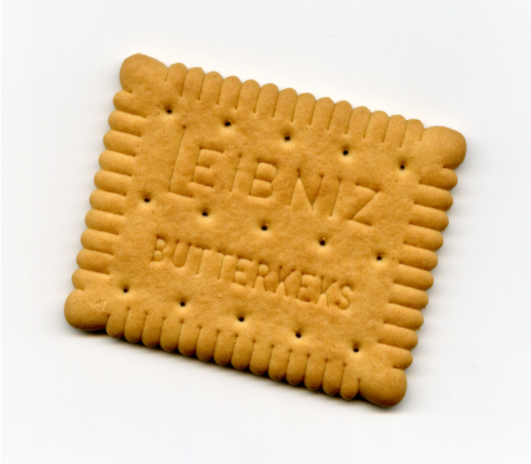
\includegraphics[scale=0.3]{Keks_original.png}
\end{center}
    \caption{Beispiel für einen Keks ohne fehlende Zähne.}
    \label{fig:keks_original}
\end{figure}\\
\newline
\textbf{{\large Fehlererkennung}}\\
\newline
Eine Möglichkeit fehlerbehaftete Ware zu erkennen, kann mit Hilfe eines Vergleichs der Bilder zwischen einem möglichst makellosen Keks (Musterbild) und des zu kontrollierenden Gebäcks (Kontrollbild) erreicht werden.\\
\newline
Zunächst muss die Ware von der Kamera erfasst werden. Hierbei kann es vorkommen, dass der Rand vom Keks nicht parallel zur Bildkante verläuft (vgl. Abb. \ref{fig:keks_original}). Die Aufnahme muss demnach entsprechend gedreht werden, damit beide Kekse miteinander verglichen werden können - ansonsten werden falsche Bereiche miteinander verarbeitet und das Ergebnis ist unbrauchbar. Je nach Fertigungsgenauigkeit kann mit Hilfe der Luftlöchern oder einer Bounding-Box am Keksrand die Orientierung der einzelnen Kekse durchgeführt werden.\\
\newline
Wenn anschließend die Aufnahme bereit zum Vergleich ist, sollen die Pixelwerte beider Bilder voneinander subtrahiert werden. Dadurch lassen sich auf einfache Weise Unterschiede erkennen. Ist beispielsweise das Kontrollbild exakt das Gleiche, wie das Musterbild, so subtrahieren sich für jeden Pixel im Bild immer die selben Werte zu 0 und es entsteht ein schwarzes Bild. Ergeben sich Unterschiede weist das resultierende Bild auf diese Stellen mit anderen Pixelwerten hin. Hierfür bieten sich  verschiedene Varianten an, z.B.:
\begin{equation}
\textbf{R} = \textbf{K} - \textbf{M}
\end{equation}
\textbf{R} $\widehat{=}$ resultierende Bildmatrix, \textbf{K} $\widehat{=}$ Bildmatrix vom Kontrollbild, \textbf{M} $\widehat{=}$ Bildmatrix vom Musterbild. \\
\newline
Wenn nach dieser Variante ein Pixelwert aus \textbf{M} größer als der korrespondierende aus \textbf{K} ist, so erhält \textbf{R} einen negativen Wert für diese Stelle. Solche Werte (also $\leq$ 0) können dann auf 0 gesetzt werden. Dies würde aber einen Informationsverlust bedeuten. Stattdessen bleibt die Information erhalten, wenn nach der Subtraktion noch der Betrag gebildet wird:
\begin{equation}
\textbf{R} = \vert \textbf{K} - \textbf{M} \vert 
\end{equation}
Je nach Anforderung kann hier weiter nach Qualitätsstufen unterteilt werden, in z.B.: fehlende Zähne oder Teig, der beim Backen übergelaufen ist. Hierfür müssen dann weitere Klassifizierungsalgorithmen auf \textbf{R} angewendet werden. Üblicherweise soll aber jeder Keks mit irgendeinem Fehler aussortiert werden. Dafür bietet sich ein einfacheres Verfahren an: der Keks soll aussortiert werden, wenn ein bestimmter Helligkeitswert überschritten worden ist, oder wenn dieser Wert eine bestimmte Anzahl überschritten wurde (mit Hilfe einer Histogrammanalyse).\\ \newline
\textbf{{\large Kamera und Umgebung}}\\
\newline
Für das zuvor beschriebene Verfahren sollte eine möglichst zweidimensionale Bildaufnahme vom Keks gemacht werden, wo keine Seitenansichten oder Schattenwürfe vorhanden sind, da bei einer seitlichen Aufnahme zu viele unbrauchbare Differenzen entstehen würden (falscher Vergleich der Bereiche im Kontroll- und Musterbild).\\
\newline
Die bevorzugte Kameraposition hierfür ist dann direkt über dem Flächenmittelpunkt des Gebäcks, mit  Blickrichtung auf die obere (und damit größte) Fläche der Ware. Die abzufotografierende Fläche muss beleuchtet werden, um den kompletten Keks analysieren zu können. Die Lichtquelle selbst sollte möglichst nah bei der Kamera platziert werden, um einen Schattenwurf zu vermeiden (ggf. mehrere Lichtquellen oder ein Flächenlicht verwenden). \\ 
\newline
\textbf{{\large Integration in den Fertigungsprozess}}\\
\newline
Die Kekse werden nacheinander, im Abstand von einer Aufnahmebreite (sodass nur ein Gebäck pro Foto aufgenommen und analysiert wird), mit Hilfe eines Förderbands an der Kamera vorbeigefahren. Um die Bildverarbeitungszeit gering zu halten, kann ein zusätzlicher Sensor (z.B.: Lichtschranke in Richtung der Gebäckkante) die Fotoaufnahme auslösen, wenn der Keks vollständig im Bildbereich liegt. Dadurch muss der Algorithmus nicht überprüfen, ob das Gebäck komplett oder nur teilweise auf der Aufnahme zu sehen ist und spart dadurch Rechenzeit. Dieser Sensor kann ebenso zur Synchronisation verwendet werden, indem er die Warenauflage auf das Förderband auslöst. Fehlerbehaftete Kekse können letztlich mit Hilfe von pneumatischen Schubzylinder vom Band geschoben werden.
\newpage
\section{Teller sind ein weites Feld (2 Bonuspunkte)}

Im Gegensatz zum ersten Aufgabenteil soll nun eine Herangehensweise entwickelt werden, bei der das zu erkennende Geschirr und dessen Umgebung vorher nicht bekannt ist.\\
\linebreak
Dies wirft verschiedene Problematiken auf. Zum Einen, kann sich gleichartiges Geschirr, je nach Hersteller und Design, voneinander stark unterscheiden. Zum Anderen, ist es sehr wahrscheinlich, dass nicht immer eine vorteilhafte Umgebung (s. Aufgabe 1) gegeben ist, was jedoch für die eigentliche Klassifizierung der Objekte unerheblich ist.\\
\linebreak
Zur Unterscheidung von Messer, Gabel und Löffel, ist es deshalb hilfreich, die Hauptträgheitsachsen zu betrachten. Das Messer ist im Gegensatz zu der Gabel und dem Löffel lang und schmal, was sich deutlich im Verhältnis der Hauptträgheitsachsen wiederspiegelt. Bei der Gabel und dem Löffel ist dieser Unterschied nicht mehr so extrem, jedoch lässt sich dort auf die gleiche Weise eine Klassifizierung vornehmen.\\
\linebreak
Die Wiedererkennung eines Tellers stellt sich in diesem Fall einfacher dar, da dieser sich durch seine Form stark vom Besteck abhebt. Die Klassifizierung über die runde Form eines Tellers (wie es in Aufgabe 1 möglich war), ist allgemein problematisch, da es sich nicht immer um runde Teller handeln muss. Auch wenn der Teller nicht rund ist, lässt sich dieser über das Verhältnis der Hauptträgheitsachsen identifizieren, da das Besteck idR. deutlich länglicher geformt ist als ein Teller. Alternativ lässt sich der Teller auch über seine verhältnismäßig große Fläche klassifizieren.\\
\linebreak
Diese unterschiedlichen Verhältnisse der Hauptträgheitsachsen, kann durch eine Ellipse verdeutlicht werden, die durch die oberen und unteren Enden dieser Achsen verläuft. Der Löffel hat idR. einen dickeren Kopf als die Gabel, wodurch die Ellipse in die Länge gezogen wird, wohingegen sie beim Messer am schmalsten, im Vergleich zum anderen Besteck, ausfällt.

%-------Text-End------------------------------------------
\end{document}

